\documentclass[../main.tex]{subfiles}
\begin{document}
\graphicspath{{../imagenes/potencia/}}
\section{Potencia}
	\subsection{Compensacion de perdida de potencia}
	A la hora de hablar de compensación, nos referimos a compensar las perdidas de un
	circuito por fuera de la carga. Recordemos que todo conductor eléctrico tiene 
	(dependiendo del conductor) propiedades inductivas, capacitivas y 
	principalmente resistivas. Nosotros nos vamos a centrar principalmente en el 
	factor resistivo y como este afecta al circuito (vamos a despreciar las 
	propiedades inductivas y capacitivas).

	En el caso de los circuitos amplificados uno puede exteriorizar por fuera del PCB, 
	su salida modificando el circuito. Ya de por si la modificación o la extensión de 
	los conductores que conducen la corriente eléctrica del Op-Amp a la carga va a 
	generar un cambio en como la potencia es disipada, ya sea en potencia activa en la 
	carga o potencia disipada o considerada ``desperdiciada'' en calor en sus 
	conductores o simplemente potencia no aprovechada en la carga, esta potencia 
	disipada por fuera de la carga tiene 2 efectos.

	El caso más sencillo para analizar estos fenómenos es teniendo una carga ``dummy'', 
	que simplemente nos importa su resistencia, sin tener en cuenta su disipación o 
	que hace con el potencial eléctrico que recibe. Esta carga esta expresada como RL 
	la cual tiene un valor de 5$\Omega$.

	En serie a la misma se coloca virtualmente una resistencia que no es parte de la 
	carga, este nuevo componente es el cual nosotros debemos compensar, llamado R1 con 
	un valor de 1$\Omega$.

	Luego tenemos nuestro Amplificador Operacional llamado AMP\_A del cual solo nos 
	importara su ganancia, y nuestra señal de entrada Signal In, la cual es una señal 
	de onda senoidal.
	
	\footnote{ Cuando uno trabaja con amplificadores se utilizan señales senoidales 
	(preferentemente de 1kHz) para analizar el comportamiento de los amplificadores 
	ya que estas, analizadas en potencia en la carga, terminan generando un valor 
	medio de potencia (Pavg) en la carga mas significativa de lo que puede ser la 
	señal de una canción por ejemplo u otro tipo de señal, además compone todos los 
	valores de tensión entre el +V y -V (valores pico a pico). Tambien es un 
	estándar que permite analizar de la misma manera a todos los amplificadores, 
	logrando comparaciones objetivas entre	dispositivos. }

	\begin{figure}[H]
		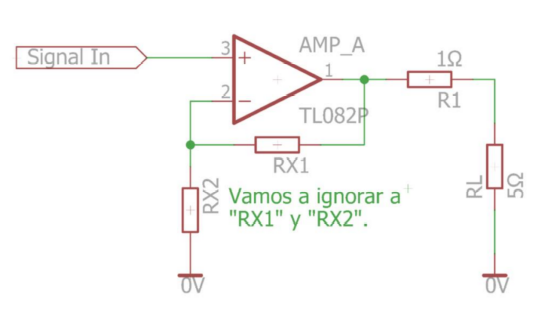
\includegraphics[width=\textwidth]{imagen1.png}
		\centering
		\caption{Circuito inicial}
	\end{figure}

	Para analizar de mejor manera los efectos de nuestro nuevo componente indeseado 
	R1, es mejor primero analizar el circuito sin este, y luego incluyéndolo para 
	realizar comparaciones y ver los efectos de este.

	\begin{figure}[H]
		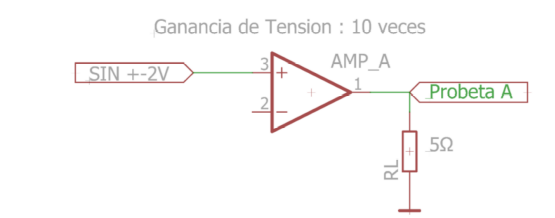
\includegraphics[width=\textwidth]{imagen2.png}
		\centering
		\caption{Circuito sin considerar R1}
	\end{figure}
	
	\begin{figure}[H]
		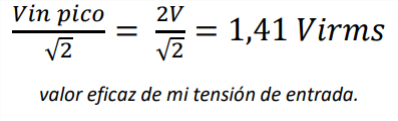
\includegraphics[width=0.7\textwidth]{imagen3.png}
		\centering
		\caption{Análisis}
	\end{figure}

	Este es el valor eficaz luego de pasar por el Op-Amp. (también podemos 
	utilizar, para amplificar, directamente a Vpico, pero siempre hay que 
	pasarlo a valor eficaz, ya que los valores pico no son los correspondientes 
	para el análisis).

	\begin{figure}[H]
		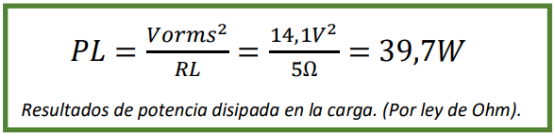
\includegraphics[width=0.7\textwidth]{imagen4.png}
		\centering
	\end{figure}

	\subsubsection*{Resultados luego de etapa de amplificación}

		\begin{figure}[H]
			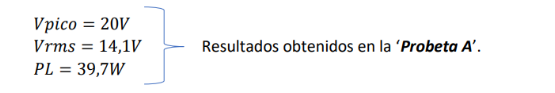
\includegraphics[width=\textwidth]{imagen5.png}
			\centering
		\end{figure}

	Como conclusión de este rápido análisis se da a conocer que en este caso la 
	totalidad de la potencia es ``aprovechada'' en la carga, no tenemos perdidas, pero 
	esto solo se daría en la situación en la cual, el amplificador se encuentre pegado 
	a la carga, o casos irreales donde nuestros conductores sean ideales y no se 
	opongan levemente a la corriente que circula por ellos.

	Ahora incluiremos en el análisis a R1 y analizaremos los valores
	\begin{figure}[H]
		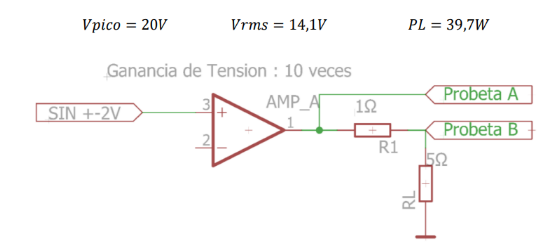
\includegraphics[width=\textwidth]{imagen6.png}
		\centering
		\caption{Circuito con R1 incluido en el análisis}
	\end{figure}
	La problemática ahora es la siguiente, la tensión que yo antes tenia 
	únicamente disipada en la carga (Probeta A $\rightarrow$ 0v), ahora esta 
	también disipada en R1, por ahora no le vamos a dar motivo a R1, sino que 
	simplemente va a ser otra resistencia ``dummy'' pero diferenciada de RL.
	Veamos como afecta R1 en la potencia en RL.

	\begin{figure}[H]
		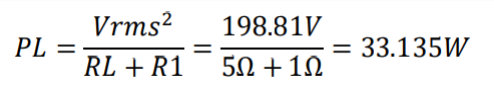
\includegraphics[width=0.7\textwidth]{imagen7.png}
		\centering
	\end{figure}
	Observación: ya de por si la propia existencia de R1, nos quita de saque ~6W 
	de Potencia total del amplificador a la carga, este es el primer efecto. Al 
	mismo tiempo, hay que tener en cuenta que aun no hemos calculado la potencia 
	en la carga, ya que estos 33,135W no son disipados únicamente en la carga, 
	sino que también en R1, por lo que R1 continúa generando cambios en el 
	circuito, esto es el segundo efecto de R1 en el circuito.
	Veamos la nueva PL, con R1.

	Para ello aplicamos un divisor de tensión a la salida del amplificador. VpA y VpB, 
	hacen referencia a las probetas ‘A’ y ‘B’ respectivamente.

	\begin{figure}[H]
		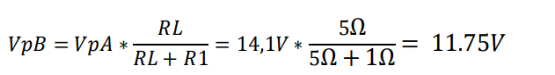
\includegraphics[width=0.7\textwidth]{imagen8.png}
		\centering
	\end{figure}

	VpB representa ahora si la caída de tensión en la carga. Con este valor podemos 
	deducir, ahora sí, PL
	\begin{figure}[H]
		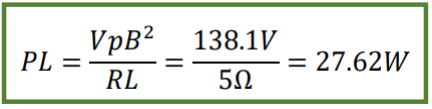
\includegraphics[width=0.7\textwidth]{imagen9.png}
		\centering
	\end{figure}

	Como se puede ver, ahora tenemos ~12W menos de lo que teníamos anteriormente de la 
	presencia de R1 disipados en la carga. Ahora a lo que viene el tema… compensaremos 
	esta perdida de potencia en R1.

	Para compensar la perdida en R1, agregaremos un nuevo componente al circuito, será 
	otro amplificador, pero que tendrá una menor ganancia, la cual debemos calcular 
	haciendo ingeniería inversa sobre el circuito. Este nuevo amplificador tendrá 
	menor impacto sobre el circuito que el amplificador A. lo único que sabemos de 
	este nuevo amplificador, llamado ``AMP\_B'' es que su ganancia será mayor a 1 e ira 
	antes del amplificador principal ‘A’ y estará trabajando con menores potenciales 
	eléctricos. Desde un punto de vista de calculo este podría estar después, pero no 
	conviene, ya que ahora ambos amplificadores estarán trabajando con potenciales 
	eléctricos grandes y deberían ser de características similares. Colocándolo antes, 
	le ahorramos trabajo a este nuevo amplificador. Este nuevo Op-Amp se llama Pre-Amp.

		\subsubsection*{Circuito resultante}
		\begin{figure}[H]
			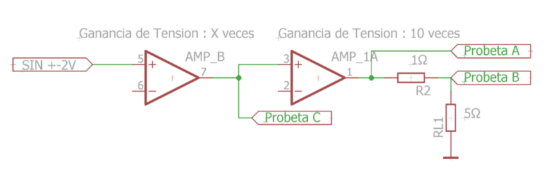
\includegraphics[width=\textwidth]{imagen10.png}
			\centering
			\caption{Circuito resultante}
		\end{figure}

	Agregamos la ``Probeta C'' para tener otro punto de análisis entre las etapas de 
	amplificación. Este valor de tensión es fundamental a la hora de calcular la 
	ganancia que debe haber en el amplificador B para recuperar la potencia en RL. 

	Sabiendo los datos tomados anteriormente, debemos ahora generar las condiciones 
	para que tengamos nuestros 39,7W nuevamente disipados en totalmente en la carga, 
	sabemos que es con un valor de tensión $V_pB$ de 14.1V (VRL).
	\[
		V_pA = VR_1 + VRL = (1\Omega \x IL_{RMS}) + 14V
	\]

	Para deducir $IL$, que es la corriente que atraviesa, a R1 y a RL en conjunto, tomaremos (al estar buscando los 14.1V en RL) que:
	\begin{figure}[H]
		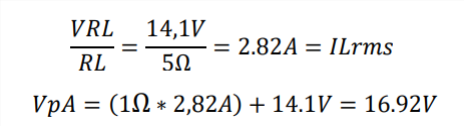
\includegraphics[width=0.7\textwidth]{imagen11.png}
		\centering
	\end{figure}

	Ahora ya con este nuevo dato de VpA, sabemos que tensión debemos tener antes de 
	la etapa de amplificación de AMP A, continuemos.
	
	A partir de esto sabiendo la ganancia de este amplificador, fija, tomada 
	anteriormente debemos proceder a hacer el inverso a la ganancia para saber la 
	tensión necesaria en la probeta ‘C’.

	\begin{figure}[H]
		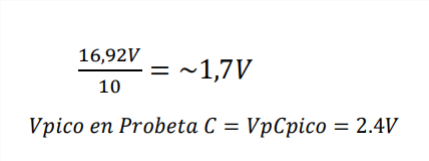
\includegraphics[width=0.7\textwidth]{imagen12.png}
		\centering
	\end{figure}

	Ya sabiendo etc... \todo{esto}

	Por ultimo debemos realizar las expresiones para deducir la ganancia en el amplificador B.

	\begin{figure}[H]
		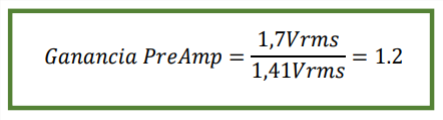
\includegraphics[width=0.7\textwidth]{imagen13.png}
		\centering
	\end{figure}

	Ese fue todo el procedimiento para compensar la perdida de potencia en R1 y 
	devolverle a la carga lo perdido con un pre amplificador. En este caso 
	tomamos a la carga como una resistencia, pero tranquilamente puede ser otra 
	cosa, como un cable. Un caso bastante común es compensar en un sistema de 
	audio, una extensión de cable de considerable longitud, este cable se 
	considera como una nueva resistencia al circuito debido a su longitud, no en 
	todos los casos este puede ser perceptible, todo dependerá la potencia 
	utilizada y el conductor.

	En el caso de que uno quiera calcular la resistencia de este cable para ver si su 
	resistencia afecta o no al circuito, a partir del largo, la sección y la 
	resistividad del conductor. el ancho de un conductor actúa como una resistencia en 
	paralelo, y la longitud como un agregado de resistencias en serie. Por ende, mayor 
	sección, menor resistencia, mayor largo, mayor resistencia.

	\begin{figure}[H]
		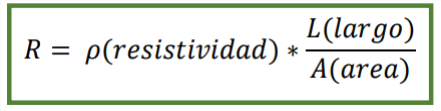
\includegraphics[width=0.7\textwidth]{imagen14.png}
		\centering
	\end{figure}
	La temperatura y la humedad son factores que tambien afectan la conductividad 
	de los conductores, estos menos significativos ( exceptuando casos extremos) 
	que la sección y el largo

	\subsection{Potencia con decibel}	
		\subsubsection{Introduccion a Decibel}
		Primero tenemos que saber que la unidad básica del decibelio es el  bel de 
		símbolo B, pero dada la amplitud de los campos que se miden en la práctica, 
		se utiliza su submúltiplo, el decibelio (dB). Es una expresión que no es 
		lineal, sino logarítmica, adimensional y matemáticamente escalar. Ni el 
		belio, ni el decibelio son unidades del Sistema internacional de unidades.

		El decibel (dB) es una unidad relativa de una señal muy utilizada por la 
		simplicidad al momento de comparar y calcular niveles de señales eléctricas. Los 
		logaritmos son muy usados debido a que la señal en decibeles (dB) puede ser 
		fácilmente sumada o restada. Estos son vistos en relaciones de tencion y de potencia. 

		La razon por la que es ventajosa el uso de dB es  la facilidad que se tiene para 
		saber si hay una atenuación o ganancia en función del signo, y además por la 
		posibilidad de hacer cálculos fáciles de suma y resta en lugar de complicadas 
		multiplicaciones y divisiones de magnitudes. A mayor valor positivo en dB, mayor 
		será la ganancia que presente el sistema, y a mayor valor negativo en dB, mayor 
		será la atenuación. Cuando el valor en dB es cero, Por ejemplo en perdida de 
		potencia, indica que la potencia de salida es igual a la de entrada.

		\subsubsection{Para calculos de perdida de potencia}
		Dado el siguente circuito
		\begin{figure}[H]
			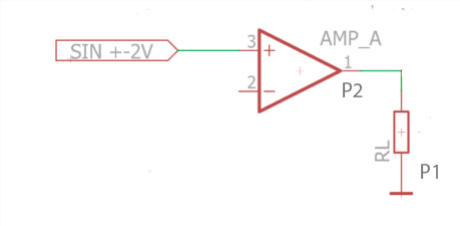
\includegraphics[width=\textwidth]{imagen15.png}
			\centering
			\caption{Circuito base}
		\end{figure}
		\[
			10\log\left(\dfrac{p_{1}}{p_{2}}\right)=dB
		\]

		Donde P2 potencia de entrada, P1 potencia de salida y dB el resultado en decibeles
		Tambien podemos hacer el calculo de decibeles de perdida con calculo de 
		tension. dado que
\begin{center}
		\(
		10\log\left(\dfrac{PL_{1}}{PL_{2}}\right)=
		10\log\left(\dfrac{\left(\dfrac{Vrms_{1}^{\ 2}}{rl}\right)}{\left(\dfrac{{Vrms_{2}}^2} {rl}\right)}\right)=
		10\log\left(\dfrac{Vrms_{1}^{\ 2}}{{Vrms_{2}}^2}\right)=
		10\log\left(\dfrac{\left(Vrms_{1}^{\ }\right)}{\left(Vrms_{2}\right)}\right)^{2}=
		2\cdot10\log\left(\dfrac{\left(Vrms_{1}^{\ }\right)} {\left(Vrms_{2}\right)}\right)=
		20\log\left(\dfrac{\left(Vrms_{1}^{\ }\right)}{\left(Vrms_{2}\right)}\right)
		\)
	\end{center}
		Donde $Vrms_1$ es tencion de salida, $Vrms2$ es tencion de entrada y Gv ganancia de tencion

	\subsection{Amplificadores de un solo extremo (SEL)}
	Para definir lo que es un amplificador de un solo extremo sería mejor explicar 
	en un inicio lo que no es. Para ello voy a dar una vaga explicación del 
	funcionamiento de los amplificadores ``push-pull'' 

	La gran mayoría de los amplificadores que no se basan en tecnología de conmutación 
	son los llamados ``amplificadores push-pull''. En estos, la potencia es manejada por 
	2 amplificadores o 2 conjuntos de estos y son utilizados en paralelo, pero 
	funcionan con polaridad invertida, de ahí que se lo llame ``push-pull''. Esto 
	permite grandes mejoras en la eficiencia en la etapa de salida, reduce las 
	distorsiones armónicas o hace ambas. Si estos amplificadores están acoplados por 
	transformador, ambos se activan en polaridad invertida y luego sus valores se 
	suman en el transformador de salida.

	Si en su lugar el diseño se encuentra en estado sólido (sin transformador), ambos 
	se complementan entre si (ósea que uno se basa en un npn y el otro es un pnp). De 
	esta forma, ambos amplificadores son controlados desde la misma fuente, pero están 
	configurados para saturarse en sentidos opuestos.

	Ambos diseños ofrecen las mismas ventajas de eficiencia y linealidad. 

	Ahora bien, en lo que se diferencia el amplificador de un solo extremo con los 
	``push-pull'' es que solo puede ``tirar'' o ``empujar'' y no ambas. Tan solo se utiliza 
	un amplificador o un conjunto de estos, lo que no genera grandes mejoras en la 
	eficiencia o una gran reducción en la distorsión. Esto puede parecer atractivo 
	gracias a su aparente ``pureza''

	Ahora si nosotros queremos representar de forma esquemática un circuito 
	amplificador de un solo extremo, representamos los amplificadores como triángulos 
	con un conector en su base al cual le conectamos la tensión a amplificar y la 
	salida en la punta del mismo, desde donde vamos a realizar la conexión a la carga. 
	Esto se hace para agilizar el diagramado y no perder tiempo ya que aquí lo que nos 
	importa no es la estructura interna del amplificador, sino su amplificación.

	\begin{figure}[H]
		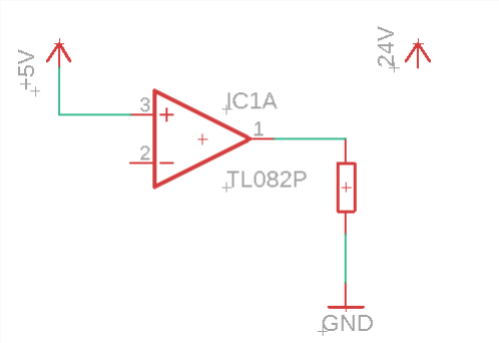
\includegraphics[width=0.85\textwidth]{imagen16.png}
		\centering
		\caption{Circuito SEL}
	\end{figure}

	En caso de que necesitemos inyectar corriente en alterna verdadera a la carga, una 
	forma de hacerlo seria utilizar una fuente de corriente continua dividida para, de 
	esta manera, centrar el punto a tierra entre + V y -V. esto puede ser nombrado 
	como fuente de energía dual. De esta forma al amplificador le llegarían, por 
	ejemplo, +10V y -10V en lugar de +20 y 0, y así  obtendríamos una CA verdadera sin 
	tener que recurrir a un transformador en la salida.

	Luego tenemos los amplificadores diferenciales que, en lugar de amplificar una 
	tensión directa, amplifica la diferencia de tensión entre su entrada de +V y -V.

	Como sabemos que esta configuración amplifica una diferencia de tensión en lugar 
	de una tensión directa, podemos decir que la tensión de salida del amplificador 
	seria igual a la diferencia de tensión entre +V y -V multiplicada por la ganancia 
	del amplificador. Pasándolo a formula quedaría:
	\[
		V_{out} = G \x V_{in} - V-{in2}
	\]

		\subsubsection*{Suponiendo el siguiente caso:}
		\begin{figure}[H]
			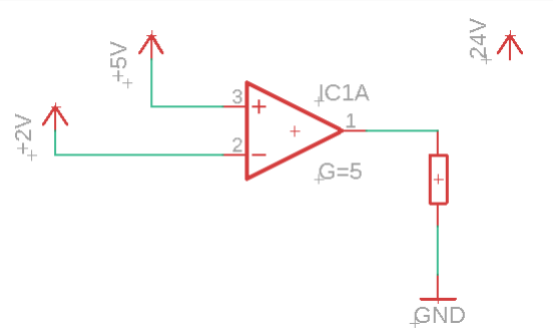
\includegraphics[width=0.85\textwidth]{imagen17.png}
			\centering
			\caption{Caso de ejemplo de SEL}
		\end{figure}
		\[
		V_{out} = 5 \x (5V - 2V = 15V
		\]

	Algunos puntos a tener en cuenta al trabajar con amplificadores es que la tensión 
	que se obtiene a la salida del amplificador nunca puede ser mayor a la tensión de 
	alimentación del mismo puesto que el amplificador no toma 5V y los transforma en 
	15V, sino que funciona como un potenciómetro que a medida que más tensión le sea 
	inyectada por las entradas, más tensión deja pasar de la alimentación a la salida

	\begin{figure}[H]
		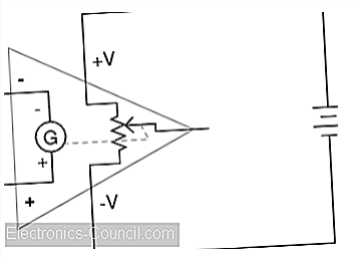
\includegraphics[width=0.4\textwidth]{imagen18.png}
		\centering
		\caption{Representación aproximada del funcionamiento de un amplificador}
		\label{fig:18}
	\end{figure}
	En la figura \ref{fig:18} se puede ver una representación aproximada del funcionamiento 
	de un amplificador donde G es un galvanómetro (un voltímetro sensible), cabe 
	aclarar que no se trata de una representación realista de la arquitectura 
	del mismo, sino que este modelo solo busca simplificar la interpretación del 
	funcionamiento de los amplificadores, y que las entradas del amplificador no 
	tienen una polaridad definida (no necesariamente deben entrar valores positivos 
	a +V ni valores negativos a -V), el amplificador simplemente toma la diferencia 
	entre las tensiones ingresadas. Aun así, debido a la relación entre las 
	entradas y las polaridades, a +V se le llama ``entrada no inversora'' y a -V se 
	le llama ``entrada inversora''.

	\begin{figure}[H]
		\centering
		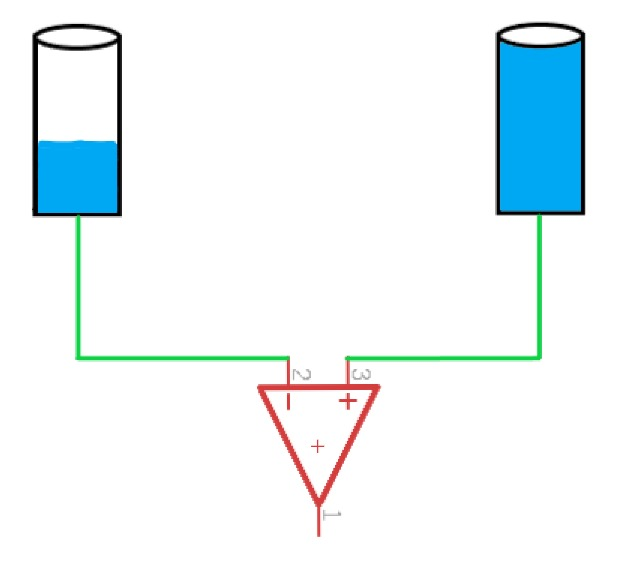
\includegraphics[width= \textwidth]{imagen20}
		\caption{Diagrama para ejemplificar el funcionamiento}
		\label{fig:20}
	\end{figure}
	En la figura \ref{fig:20} se puede ver el motivo de esto. Si ingresamos valores de tensión mayores 
	a -V y menores a +V nuestro amplificador entregara valores tensión con 
	polaridad negativa ya que este solo toma la diferencia de potencial entre 
	sus 2 entradas e ignora la diferencia entre cualquiera de estas y la 
	conexión a tierra. Esto nos permite utilizarlo en diferentes aplicaciones a 
	modo de comparador midiendo la polaridad del potencial de salida. 

	Por ejemplo, supongamos que tenemos 2 tanques con agua y queremos saber cual tiene 
	más, para esto podríamos hacer un circuito con un amplificador diferencial y de 
	esa forma obtener que tanque tiene mayor cantidad de agua viendo la polaridad del 
	potencial de salida de nuestro amplificador e incluso podríamos saber de cuanta 
	diferencia estamos hablando observado la tensión de salida del amplificador. Cabe 
	aclarar que para esto tenemos que estar al tanto de cuanto se amplificara la 
	tensión, saber que tanque esta conectado a cada input y tenemos que sacar una 
	proporcionalidad entre la tensión y la cantidad de agua de la que hablamos.

	\begin{figure}[H]
		\centering
		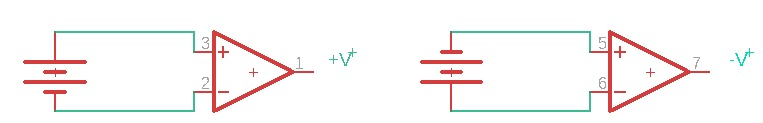
\includegraphics[width= \textwidth]{imagen21}
	\end{figure}
	Suponiendo que nosotros hayamos armado nuestro circuito para que entregue un 
	volt por litro, que nuestro amplificador amplifica por 2 veces y que el primer 
	tanque tiene 2 litros y el segundo 3, obtendríamos que a la salida tendríamos 
	+2V de forma que podemos saber que el tanque de la derecha es el más cargado ya 
	que es el que esta conectado a +V y dividiendo la tensión por la ganancia del 
	amplificador podemos sacar de cuantos litros de diferencia estaríamos hablando, 
	que en este caso seria 1L. obviamente, la imagen es completamente conceptual y 
	solo busca expresar el ejemplo de forma más visual.

	Para el circuito de control automático básico se suele comparar la variable de 
	proceso con un punto de referencia en base al cual se mide la diferencia entre 
	estos y de esta forma, tomar acciones dependientes de la diferencia

	\subsection{Bridge-Tied Load (BTL)}
	Una carga atada a un puente es una configuración de salida para amplificadores de 
	audio, una forma de puente de impedancia que se utiliza principalmente en 
	aplicaciones de audio para automóviles. Los dos canales de un amplificador estéreo 
	reciben la misma señal de audio monoaural, con la polaridad eléctrica de un canal 
	invertido. Un altavoz está conectado entre las dos salidas del amplificador, 
	puenteando los terminales de salida. Esto duplica la oscilación de tensión 
	disponible en la carga en comparación con el mismo amplificador utilizado sin 
	puente. La configuración se usa con mayor frecuencia para subwoofers.

	Para una variación de tensión de salida dada, cuanto menor sea la impedancia, 
	mayor será la carga del amplificador. El puenteo se usa para permitir que un 
	amplificador impulse cargas bajas a una potencia más alta, porque la potencia es 
	inversamente proporcional a la impedancia y proporcional al cuadrado del voltaje, 
	de acuerdo con la ecuación P = V2 / R . Esta ecuación también muestra que el 
	puente cuadriplica la potencia teórica en un amplificador, sin embargo, esto es 
	cierto solo para cargas lo suficientemente bajas. Por ejemplo, para cargas en las 
	que el amplificador alcanza su máximo potencial en el modo de un solo extremo, no 
	se puede obtener ninguna ganancia con el puente. Esto se debe a que un 
	amplificador puede tener limitaciones de corriente o, en aplicaciones prácticas, 
	una disipación de calor y una fuente de alimentación inadecuadas.

		\subsubsection{Circuito}
		La imagen muestra dos amplificadores A1 y A2 idénticos conectados en modo puente.

		\begin{figure}[H]
			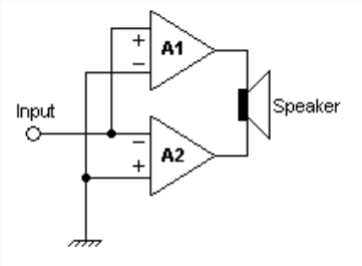
\includegraphics[width=0.8\textwidth]{imagen19.png}
			\centering
		\end{figure}

		El sistema está dispuesto de tal manera que las salidas de los 
		amplificadores estén invertidas entre sí. En otras palabras, como la señal 
		en un amplificador oscila positivamente, la señal en el otro oscila 
		negativamente.

		Cuando la salida de un amplificador es de +10V, la salida del 
		otro será de -10V y viceversa. La carga está conectada entre las salidas 
		"calientes" de los dos amplificadores y está sujeta a la diferencia de 
		potencial entre ellos. 
		
		Si el potencial instantáneo en la salida de un 
		amplificador es de +10V, entonces la salida del otro será de -10V y la 
		diferencia de potencial a través de la carga será de 20V, o el doble del 
		potencial disponible de un solo amplificador.

		\subsubsection{Ventajas y desventajas:}
		Dado que se utilizan dos amplificadores en polaridad opuesta, utilizando la misma 
		fuente de alimentación, la salida en puente es flotante. Esto hace que un 
		condensador de bloqueo de CC entre el amplificador y la carga sea innecesario, 
		ahorrando costos y espacio y evitando la reducción de potencia a baja frecuencia 
		debido al condensador.  Por la misma razón, las salidas del amplificador nunca 
		deben conectarse a tierra o puede dañar el amplificador. El factor de 
		amortiguación se reduce a la mitad, lo que es beneficioso para la entrega de potencia.

		Conectar un amplificador aumenta la potencia que se puede suministrar a un 
		altavoz, pero no aumenta la potencia total disponible del amplificador. Debido a 
		que un amplificador puente funciona en modo mono, se requiere un segundo 
		amplificador idéntico para el funcionamiento estéreo. 

		\subsubsection{Consideraciones sobre el diseño del amplificador:}
		Hay quienes afirman que operar el par estéreo de un amplificador en modo puente 
		entregará cuatro veces la potencia de uno de los canales del par. Dada una carga 
		equivalente, la potencia entregada es proporcional al cuadrado de la tensión y el 
		funcionamiento en modo puente duplica la tensión presentada. Sobre esa base, un 
		par de canales de amplificador operados en modo puente deberían entregar cuatro 
		veces la potencia de un solo amplificador, impulsando la misma carga. Sin embargo, 
		esto ignora una consideración importante de que debido a que la diferencia de 
		potencial en la carga se duplica, la corriente que pasa a través de la carga (y a 
		través de cada una de las salidas del amplificador) también se duplicará.

		Los circuitos amplificadores se diseñan típicamente con los componentes de menor 
		costo necesarios para proporcionar las características de rendimiento deseadas. 
		Los componentes que transportan la corriente de salida del amplificador tenderán a 
		ser los más pequeños (más baratos) que satisfarán el consumo de corriente pico 
		cuando el amplificador esté funcionando a la máxima potencia, en el modo de 
		operación diseñado. Operar un amplificador diseñado para operación en solitario en 
		modo puente significará que la corriente en los componentes que impulsan la salida 
		podría alcanzar un pico del doble de lo que fueron diseñados originalmente.

		Si los componentes pueden hacer frente a la corriente adicional más allá de la 
		corriente máxima esperada para el funcionamiento en solitario, entonces se podría 
		lograr una mayor entrega de energía. Pero en el caso general, solo se puede 
		esperar que el amplificador funcione como se especifica, y operarlo más allá de la 
		especificación dará lugar a un mayor riesgo de daño permanente al circuito del 
		amplificador.

		Como tal, si un amplificador diseñado para operación en solitario se va a 
		reutilizar para operación en modo puente, la impedancia de carga debe duplicarse. 
		Esto debería significar que el consumo de corriente permanece dentro de los 
		límites del diseño del amplificador. En este escenario, la potencia entregada por 
		el par de amplificadores puenteados será el doble de la potencia entregada por un 
		solo canal de amplificador.

		Pero en algunos escenarios, los amplificadores están diseñados particularmente 
		para operar en modo puente. Dichos amplificadores fueron hechos específicamente 
		para poder suministrar la corriente necesaria. En tales sistemas, el par en puente 
		podrá entregar cuatro veces esa potencia que un solo canal de amplificador habría 
		podido entregar. La opción del modo puente se usa a menudo en sistemas de 
		megafonía y especialmente en aplicaciones de audio para automóviles para alimentar 
		altavoces de graves a alta potencia.

\end{document}
